% answers.tex —— 2013 年·天津卷·文科 · 参考答案与详细解析片段
% 由 tools/generate_projects.py 依来源总账自 2013/2013_数学真题_天津文_试题.md + 2013/2013_数学真题_天津文_解析正文.md + 2013/2013_数学真题_天津文_答案要点.md 生成，勿手改（改源 MD 后重跑）

\begin{answer}
\gksolhead{1}{}

\textbf{题目}：

已知集合 $A=\{x\in\mathbf R\mid |x|\leqslant2\}$，$B=\{x\in\mathbf R\mid x\leqslant1\}$，则 $A\cap B=$\mbox{（　　）}

（A）$(-\infty,2]$；（B）$[1,2]$；（C）$[-2,2]$；（D）$[-2,1]$。

\Needspace{4\baselineskip}
\textbf{解析}
\Needspace{5\baselineskip}
$|x|\leqslant2\iff-2\leqslant x\leqslant2$，故
\nopagebreak[4]
\[A=[-2,2],\qquad B=(-\infty,1].\]
\Needspace{5\baselineskip}
在数轴上取公共部分：
\nopagebreak[4]
\[A\cap B=[-2,1].\]
选 D。

\gkanswer{答案：D。}

\end{answer}
\begin{answer}
\gksolhead{2}{}

\textbf{题目}：

设变量 $x$，$y$ 满足约束条件 $\begin{cases}3x+y-6\geqslant0,\\ x-y-2\leqslant0,\\ y-3\leqslant0,\end{cases}$ 则目标函数 $z=y-2x$ 的最小值为\mbox{（　　）}

（A）$-7$；（B）$-4$；（C）$1$；（D）$2$。

\Needspace{4\baselineskip}
\textbf{解析}
\Needspace{5\baselineskip}
三条边界直线分别为 $3x+y-6=0$，$x-y-2=0$，$y-3=0$。两两求交点：
\nopagebreak[4]
\[\begin{aligned}
3x+y-6=0,\ y-3=0 &\Longrightarrow (1,3);\\
3x+y-6=0,\ x-y-2=0 &\Longrightarrow (2,0);\\
x-y-2=0,\ y-3=0 &\Longrightarrow (5,3).
\end{aligned}\]
\Needspace{5\baselineskip}
将三点代入检验，均满足三个不等式，故可行域是以 $(1,3)$，$(2,0)$，$(5,3)$ 为顶点的三角形（含边界）。$z=y-2x$ 为线性函数，最值必在顶点处取到：
\nopagebreak[4]
\[z(1,3)=3-2=1,\qquad z(2,0)=0-4=-4,\qquad z(5,3)=3-10=-7.\]
故 $z_{\min}=-7$（在点 $(5,3)$ 处取得）。选 A。

\gkanswer{答案：A。}

\end{answer}
\begin{answer}
\gksolhead{3}{}

\textbf{题目}：

阅读如图所示的程序框图，运行相应的程序，则输出 $n$ 的值为\mbox{（　　）}
\nopagebreak[4]
\begin{center}% 2013 天津卷文科第 3 题：输出 n 的值的程序框图。
\begin{tikzpicture}[font=\footnotesize, >=Stealth, line width=0.45pt,
  node distance=4.6mm,
  term/.style={draw, rounded corners=5pt, minimum height=1.9em, inner xsep=9pt},
  io/.style={draw, trapezium, trapezium left angle=72, trapezium right angle=108,
             minimum height=1.9em, inner xsep=8pt},
  box/.style={draw, minimum height=1.9em, inner xsep=7pt},
  dec/.style={draw, diamond, aspect=2.9, inner sep=1pt}]
  \node[term] (start) {开始};
  \node[box, below=5mm of start] (init) {$n=1$，$S=0$};
  \node[box, below=7mm of init] (acc) {$S=S+(-1)^n\cdot n$};
  \node[dec, below=6mm of acc] (test) {$S\geqslant2$?};
  \node[box, right=12mm of test] (inc) {$n=n+1$};
  \node[io, below=9mm of test] (output) {输出 $n$};
  \node[term, below=5mm of output] (end) {结束};
  \draw[->] (start) -- (init);
  \draw[->] (init) -- (acc);
  \draw[->] (acc) -- (test);
  \draw[->] (test) -- node[right] {是} (output);
  \draw[->] (test.east) -- node[above] {否} (inc.west);
  \draw[->] (output) -- (end);
  % 否分支：n=n+1 后绕回累加框上方，再向下进入累加框
  \coordinate (top) at ($(acc.north)+(0,6mm)$);
  \coordinate (back) at ($(acc.north)+(1.15,0)$);
  \draw[->] (inc.north) -- (inc.north |- top) -- (back |- top) -- (back);
\end{tikzpicture}
\end{center}
\nopagebreak[4]
（A）$7$；（B）$6$；（C）$5$；（D）$4$。

\Needspace{4\baselineskip}
\textbf{解析}
框图顺序为：先执行 $S=S+(-1)^n\cdot n$，再判断 $S\geqslant2$；不成立时 $n$ 增加 $1$ 并返回累加框。逐次计算：

\begin{center}
\begin{tabular}{llll}
\toprule
轮次 & 累加前 $(n,S)$ & 累加后 $S$ & $S\geqslant2$ \\
\midrule
1 & $(1,0)$ & $0+(-1)^1\times1=-1$ & 否，$n\to2$ \\
2 & $(2,-1)$ & $-1+(-1)^2\times2=1$ & 否，$n\to3$ \\
3 & $(3,1)$ & $1+(-1)^3\times3=-2$ & 否，$n\to4$ \\
4 & $(4,-2)$ & $-2+(-1)^4\times4=2$ & 是，输出 $n=4$ \\
\bottomrule
\end{tabular}
\end{center}

故输出的 $n$ 的值为 $4$。选 D。

\gkanswer{答案：D。}

\end{answer}
\begin{answer}
\gksolhead{4}{}

\textbf{题目}：

设 $a$，$b\in\mathbf R$，则“$(a-b)\cdot a^2<0$”是“$a<b$”的\mbox{（　　）}

（A）充分而不必要条件；（B）必要而不充分条件；（C）充要条件；（D）既不充分也不必要条件。

\Needspace{4\baselineskip}
\textbf{解析}
\Needspace{5\baselineskip}
因 $a^2\geqslant0$，故
\nopagebreak[4]
\[(a-b)\cdot a^2<0\iff a^2>0\ \text{\text{且}}\ a-b<0\iff a\neq0\ \text{\text{且}}\ a<b.\]
所以“$(a-b)a^2<0$”能推出“$a<b$”，是充分条件。

反之，取 $a=0$，$b=1$，此时 $a<b$，但 $(a-b)a^2=(-1)\times0=0$，不满足 $(a-b)a^2<0$，故不是必要条件。

因此是充分而不必要条件。选 A。

\gkanswer{答案：A。}

\end{answer}
\begin{answer}
\gksolhead{5}{}

\textbf{题目}：

已知过点 $P(2,2)$ 的直线与圆 $(x-1)^2+y^2=5$ 相切，且与直线 $ax-y+1=0$ 垂直，则 $a=$\mbox{（　　）}

（A）$-\dfrac12$；（B）$1$；（C）$2$；（D）$\dfrac12$。

\Needspace{4\baselineskip}
\textbf{解析}
点 $P(2,2)$ 到圆心 $(1,0)$ 的距离为 $\sqrt{(2-1)^2+2^2}=\sqrt5$，等于半径，故 $P$ 在圆上，过 $P$ 的切线只有一条。

\Needspace{5\baselineskip}
设切线为 $y-2=k(x-2)$，即 $kx-y+(2-2k)=0$。由圆心到切线的距离等于半径：
\nopagebreak[4]
\[\frac{|k\cdot1-0+2-2k|}{\sqrt{k^2+1}}=\sqrt5\Longrightarrow(2-k)^2=5(k^2+1).\]
\Needspace{5\baselineskip}
展开得
\nopagebreak[4]
\[4-4k+k^2=5k^2+5\Longrightarrow4k^2+4k+1=0\Longrightarrow(2k+1)^2=0\Longrightarrow k=-\frac12.\]
\Needspace{5\baselineskip}
直线 $ax-y+1=0$ 的斜率为 $a$，两直线垂直，故
\nopagebreak[4]
\[a\cdot\left(-\frac12\right)=-1\Longrightarrow a=2.\]
选 C。

\gkanswer{答案：C。}

\end{answer}
\begin{answer}
\gksolhead{6}{}

\textbf{题目}：

函数 $f(x)=\sin\left(2x-\dfrac\pi4\right)$ 在区间 $\left[0,\dfrac\pi2\right]$ 上的最小值为\mbox{（　　）}

（A）$-1$；（B）$-\dfrac{\sqrt2}2$；（C）$\dfrac{\sqrt2}2$；（D）$0$。

\Needspace{4\baselineskip}
\textbf{解析}
\Needspace{5\baselineskip}
令 $t=2x-\dfrac\pi4$。当 $x\in\left[0,\dfrac\pi2\right]$ 时，$2x\in[0,\pi]$，故
\nopagebreak[4]
\[t\in\left[-\frac\pi4,\ \frac{3\pi}4\right].\]
\Needspace{5\baselineskip}
在该区间上 $\sin t$ 先增后减，且
\nopagebreak[4]
\[\sin\left(-\frac\pi4\right)=-\frac{\sqrt2}2<\frac{\sqrt2}2=\sin\frac{3\pi}4,\qquad \max\sin t=\sin\frac\pi2=1.\]
故最小值在左端点 $t=-\dfrac\pi4$（即 $x=0$）处取得，为 $-\dfrac{\sqrt2}2$。选 B。

\gkanswer{答案：B。}

\end{answer}
\begin{answer}
\gksolhead{7}{}

\textbf{题目}：

已知函数 $f(x)$ 是定义在 $\mathbf R$ 上的偶函数，且在区间 $[0,+\infty)$ 上单调递增。若实数 $a$ 满足 $f(\log_2 a)+f\left(\log_{\frac12}a\right)\leqslant2f(1)$，则 $a$ 的取值范围是\mbox{（　　）}

（A）$[1,2]$；（B）$\left(0,\dfrac12\right]$；（C）$\left[\dfrac12,2\right]$；（D）$(0,2]$。

\Needspace{4\baselineskip}
\textbf{解析}
\Needspace{5\baselineskip}
由换底关系 $\log_{\frac12}a=\dfrac{\log_2 a}{\log_2\frac12}=-\log_2 a$。记 $t=\log_2 a$，由 $f$ 为偶函数得 $f(-t)=f(t)$，于是条件化为
\nopagebreak[4]
\[f(t)+f(-t)\leqslant2f(1)\Longrightarrow2f(t)\leqslant2f(1)\Longrightarrow f(t)\leqslant f(1).\]
\Needspace{5\baselineskip}
因 $f$ 在 $[0,+\infty)$ 上单调递增且为偶函数，故 $f(t)=f(|t|)$ 且 $f(|t|)\leqslant f(1)\iff|t|\leqslant1$，即
\nopagebreak[4]
\[|\log_2 a|\leqslant1\Longrightarrow-1\leqslant\log_2 a\leqslant1\Longrightarrow\frac12\leqslant a\leqslant2.\]
又 $a>0$ 已含于该区间。故 $a\in\left[\dfrac12,2\right]$。选 C。

\gkanswer{答案：C。}

\end{answer}
\begin{answer}
\gksolhead{8}{}

\textbf{题目}：

设函数 $f(x)=\mathrm e^x+x-2$，$g(x)=\ln x+x^2-3$。若实数 $a$，$b$ 满足 $f(a)=0$，$g(b)=0$，则\mbox{（　　）}

（A）$g(a)<0<f(b)$；（B）$f(b)<0<g(a)$；（C）$0<g(a)<f(b)$；（D）$f(b)<g(a)<0$。

\Needspace{4\baselineskip}
\textbf{解析}
\Needspace{5\baselineskip}
$f'(x)=\mathrm e^x+1>0$，故 $f$ 在 $\mathbf R$ 上单调递增；又
\nopagebreak[4]
\[f(0)=1+0-2=-1<0,\qquad f(1)=\mathrm e+1-2=\mathrm e-1>0,\]
故 $f(a)=0$ 的根 $a\in(0,1)$。

\Needspace{5\baselineskip}
当 $x>0$ 时 $g'(x)=\dfrac1x+2x>0$，故 $g$ 在 $(0,+\infty)$ 上单调递增；又
\nopagebreak[4]
\[g(1)=0+1-3=-2<0,\qquad g(2)=\ln2+4-3=\ln2+1>0,\]
故 $g(b)=0$ 的根 $b\in(1,2)$。

\Needspace{5\baselineskip}
于是 $a<1<b$。由 $g$ 递增得 $g(a)<g(1)=-2<0$；由 $f$ 递增得 $f(b)>f(1)=\mathrm e-1>0$。所以
\nopagebreak[4]
\[g(a)<0<f(b).\]
选 A。

\gkanswer{答案：A。}

\end{answer}
\begin{answer}
\gksolhead{9}{}

\textbf{题目}：

$\mathrm i$ 是虚数单位，复数 $(3+\mathrm i)(1-2\mathrm i)=$\gkblank{}。

\Needspace{4\baselineskip}
\textbf{解析}
\Needspace{5\baselineskip}
按复数乘法展开，注意 $\mathrm i^2=-1$：
\nopagebreak[4]
\[(3+\mathrm i)(1-2\mathrm i)=3-6\mathrm i+\mathrm i-2\mathrm i^2=3-5\mathrm i+2=5-5\mathrm i.\]
填 $5-5\mathrm i$。

\gkanswer{答案：$5-5\mathrm i$。}

\end{answer}
\begin{answer}
\gksolhead{10}{}

\textbf{题目}：

已知一个正方体的所有顶点在一个球面上，若球的体积为 $\dfrac{9\pi}2$，则正方体的棱长为\gkblank{}。

\Needspace{4\baselineskip}
\textbf{解析}
正方体的八个顶点都在球面上，故球为正方体的外接球，球的直径等于正方体的体对角线。

\Needspace{5\baselineskip}
由 $V=\dfrac43\pi R^3=\dfrac{9\pi}2$ 得
\nopagebreak[4]
\[R^3=\frac{9\pi}2\cdot\frac3{4\pi}=\frac{27}8\Longrightarrow R=\frac32\Longrightarrow 2R=3.\]
\Needspace{5\baselineskip}
设棱长为 $a$，体对角线为 $\sqrt3a$，故
\nopagebreak[4]
\[\sqrt3a=3\Longrightarrow a=\sqrt3.\]
填 $\sqrt3$。

\gkanswer{答案：$\sqrt3$。}

\end{answer}
\begin{answer}
\gksolhead{11}{}

\textbf{题目}：

已知抛物线 $y^2=8x$ 的准线过双曲线 $\dfrac{x^2}{a^2}-\dfrac{y^2}{b^2}=1$（$a>0$，$b>0$）的一个焦点，且双曲线的离心率为 $2$，则该双曲线的方程为\gkblank{}。

\Needspace{4\baselineskip}
\textbf{解析}
抛物线 $y^2=8x$ 的准线为 $x=-2$。

双曲线焦点在 $x$ 轴上，坐标为 $(\pm c,0)$，$c=\sqrt{a^2+b^2}$。准线 $x=-2$ 过其中一个焦点，故 $c=2$。

\Needspace{5\baselineskip}
又离心率 $e=\dfrac ca=2$，得 $a=1$，于是
\nopagebreak[4]
\[b^2=c^2-a^2=4-1=3.\]
故双曲线方程为 $x^2-\dfrac{y^2}3=1$。填 $x^2-\dfrac{y^2}3=1$。

\gkanswer{答案：$x^2-\dfrac{y^2}3=1$。}

\end{answer}
\begin{answer}
\gksolhead{12}{}

\textbf{题目}：

在平行四边形 $ABCD$ 中，$AD=1$，$\angle BAD=60^\circ$，$E$ 为 $CD$ 的中点。若 $\overrightarrow{AC}\cdot\overrightarrow{BE}=1$，则 $AB$ 的长为\gkblank{}。

\Needspace{4\baselineskip}
\textbf{解析}
\Needspace{5\baselineskip}
记 $\overrightarrow{AB}=\mathbf u$，$\overrightarrow{AD}=\mathbf v$，设 $|\mathbf u|=x$。则 $|\mathbf v|=1$，
\nopagebreak[4]
\[\mathbf u\cdot\mathbf v=x\cdot1\cdot\cos60^\circ=\frac x2.\]
\Needspace{5\baselineskip}
由 $E$ 为 $CD$ 的中点，$\overrightarrow{CE}=\dfrac12\overrightarrow{CD}=-\dfrac12\mathbf u$，故
\nopagebreak[4]
\[\overrightarrow{AC}=\mathbf u+\mathbf v,\qquad \overrightarrow{BE}=\overrightarrow{BC}+\overrightarrow{CE}=\mathbf v-\frac12\mathbf u.\]
\Needspace{5\baselineskip}
于是
\nopagebreak[4]
\[\overrightarrow{AC}\cdot\overrightarrow{BE}=(\mathbf u+\mathbf v)\cdot\left(\mathbf v-\frac12\mathbf u\right)
=\mathbf u\cdot\mathbf v-\frac12|\mathbf u|^2+|\mathbf v|^2-\frac12\mathbf v\cdot\mathbf u
=\frac12\cdot\frac x2-\frac{x^2}2+1.\]
\Needspace{5\baselineskip}
由题设该值为 $1$：
\nopagebreak[4]
\[\frac x4-\frac{x^2}2+1=1\Longrightarrow\frac x4-\frac{x^2}2=0\Longrightarrow x\left(\frac14-\frac x2\right)=0.\]
因 $x>0$，故 $x=\dfrac12$，即 $AB=\dfrac12$。填 $\dfrac12$。

\gkanswer{答案：$\dfrac12$。}

\end{answer}
\begin{answer}
\gksolhead{13}{}

\textbf{题目}：

如图，在圆内接梯形 $ABCD$ 中，$AB\parallel DC$，过点 $A$ 作圆的切线与 $CB$ 的延长线交于点 $E$。若 $AB=AD=5$，$BE=4$，则弦 $BD$ 的长为\gkblank{}。
\nopagebreak[4]
\begin{center}% 2013 天津卷文科第 13 题：圆内接梯形 ABCD（AB∥DC），AE 为过 A 的切线，
% 与 CB 的延长线交于 E。坐标按 AB=AD=5、BE=4 精确计算：
% A(3.75,-3.307)、B(7.5,0)、C(4.6875,4.134)、D(0,0)、E(9.75,-3.307)，
% 外接圆圆心 (3.75,0.4727)、半径 3.7797（A 为圆的最低点，故切线水平）。
\begin{tikzpicture}[font=\footnotesize, line width=0.5pt, scale=0.62,
  dot/.style={circle, fill=black, inner sep=1.1pt}]
  \coordinate (D) at (0,0);
  \coordinate (B) at (7.5,0);
  \coordinate (C) at (4.6875,4.1338);
  \coordinate (A) at (3.75,-3.3072);
  \coordinate (E) at (9.75,-3.3072);
  \coordinate (O) at (3.75,0.4727);
  \draw (O) circle (3.7797);
  % 梯形四边
  \draw (C) -- (D);
  \draw (D) -- (A);
  \draw (A) -- (B);
  \draw (B) -- (C);
  % 对角线
  \draw (D) -- (B);
  % CB 的延长线过 B 到 E，AE 为切线
  \draw (C) -- (E);
  \draw (A) -- ($(A)!-0.13!(E)$);
  \draw (A) -- (E);
  \foreach \p in {A,B,C,D,E} \node[dot] at (\p) {};
  \node[above left=-1pt] at (C) {$C$};
  \node[left=-1pt] at (D) {$D$};
  \node[above right=-1pt] at (B) {$B$};
  \node[below] at (A) {$A$};
  \node[right] at (E) {$E$};
\end{tikzpicture}
\end{center}
\nopagebreak[4]
\Needspace{4\baselineskip}
\textbf{解析}
圆内接梯形必为等腰梯形：由 $AB\parallel DC$ 得 $\angle DAB+\angle ADC=180^\circ$，又 $ABCD$ 内接于圆得 $\angle ABC+\angle ADC=180^\circ$，故 $\angle DAB=\angle ABC$，从而 $AD=BC$。已知 $AD=5$，故 $BC=5$。

\Needspace{5\baselineskip}
$E$ 在 $CB$ 的延长线上，故 $C$，$B$，$E$ 共线且
\nopagebreak[4]
\[CE=CB+BE=5+4=9.\]
\Needspace{5\baselineskip}
由切割线定理（$EA$ 为切线，$EBC$ 为割线）：
\nopagebreak[4]
\[EA^2=EB\cdot EC=4\times9=36\Longrightarrow EA=6.\]
\Needspace{5\baselineskip}
在 $\triangle ABE$ 中，$AB=5$，$BE=4$，$AE=6$，由余弦定理
\nopagebreak[4]
\[\cos\angle ABE=\frac{AB^2+BE^2-AE^2}{2\cdot AB\cdot BE}=\frac{25+16-36}{2\times5\times4}=\frac18.\]
\Needspace{5\baselineskip}
因 $\angle ABC$ 与 $\angle ABE$ 互补，
\nopagebreak[4]
\[\cos\angle ABC=-\frac18.\]
\Needspace{5\baselineskip}
在 $\triangle ABC$ 中，$AB=5$，$BC=5$，
\nopagebreak[4]
\[AC^2=AB^2+BC^2-2\cdot AB\cdot BC\cos\angle ABC=25+25-2\times25\times\left(-\frac18\right)=\frac{225}4,\]
\Needspace{5\baselineskip}
故 $AC=\dfrac{15}2$。等腰梯形的两条对角线相等，故
\nopagebreak[4]
\[BD=AC=\frac{15}2.\]
填 $\dfrac{15}2$。

\gkanswer{答案：$\dfrac{15}2$。}

\end{answer}
\begin{answer}
\gksolhead{14}{}

\textbf{题目}：

设 $a+b=2$，$b>0$，则 $\dfrac1{2|a|}+\dfrac{|a|}b$ 的最小值为\gkblank{}。

\Needspace{4\baselineskip}
\textbf{解析}
由 $b=2-a>0$ 得 $a<2$，且 $a\neq0$（否则 $\dfrac1{2|a|}$ 无意义）。按 $a$ 的符号分两类。

\Needspace{5\baselineskip}
\textbf{（i）当 $a>0$ 时}，$0<a<2$，原式为
\nopagebreak[4]
\[T=\frac1{2a}+\frac a{2-a}.\]
\Needspace{5\baselineskip}
因 $4a(2-a)>0$，作差
\nopagebreak[4]
\[\begin{aligned}
4a(2-a)\left(T-\frac54\right)&=2(2-a)+4a^2-5a(2-a)\\
&=4-2a+4a^2-10a+5a^2\\
&=9a^2-12a+4=(3a-2)^2\geqslant0,
\end{aligned}\]
故 $T\geqslant\dfrac54$，等号在 $a=\dfrac23$（此时 $b=\dfrac43$）处成立。

\Needspace{5\baselineskip}
\textbf{（ii）当 $a<0$ 时}，令 $t=-a>0$，则 $b=2+t$，原式为
\nopagebreak[4]
\[T=\frac1{2t}+\frac t{2+t}.\]
\Needspace{5\baselineskip}
因 $4t(2+t)>0$，作差
\nopagebreak[4]
\[4t(2+t)\left(T-\frac34\right)=2(2+t)+4t^2-3t(2+t)=4+2t+4t^2-6t-3t^2=t^2-4t+4=(t-2)^2\geqslant0,\]
故 $T\geqslant\dfrac34$，等号在 $t=2$，即 $a=-2$，$b=4$ 处成立。

比较两类的最小值，$\dfrac34<\dfrac54$，故原式的最小值为 $\dfrac34$（此时 $a=-2$，$b=4$）。填 $\dfrac34$。

\gkanswer{答案：$\dfrac34$。}

\end{answer}
\begin{answer}
\gksolhead{15}{}

\textbf{题目}：

某产品的三个质量指标分别为 $x$，$y$，$z$，用综合指标 $S=x+y+z$ 评价该产品的等级。若 $S\leqslant4$，则该产品为一等品。现从一批该产品中，随机抽取 $10$ 件产品作为样本，其质量指标列表如下：

\begin{center}
\begin{tabular}{llllll}
\toprule
产品编号 & $A_1$ & $A_2$ & $A_3$ & $A_4$ & $A_5$ \\
\midrule
质量指标 $(x,y,z)$ & $(1,1,2)$ & $(2,1,1)$ & $(2,2,2)$ & $(1,1,1)$ & $(1,2,1)$ \\
产品编号 & $A_6$ & $A_7$ & $A_8$ & $A_9$ & $A_{10}$ \\
质量指标 $(x,y,z)$ & $(1,2,2)$ & $(2,1,1)$ & $(2,2,1)$ & $(1,1,1)$ & $(2,1,2)$ \\
\bottomrule
\end{tabular}
\end{center}

（1） 利用上表提供的样本数据估计该批产品的一等品率；

（2） 在该样本的一等品中，随机抽取 $2$ 件产品。
① 用产品编号列出所有可能的结果；
② 设事件 $B$ 为“在取出的 $2$ 件产品中，每件产品的综合指标 $S$ 都等于 $4$”，求事件 $B$ 发生的概率。

\Needspace{4\baselineskip}
\textbf{解析}
\textbf{（1）} 逐个计算综合指标 $S=x+y+z$：

\begin{center}
\begin{tabular}{llllll}
\toprule
编号 & $A_1$ & $A_2$ & $A_3$ & $A_4$ & $A_5$ \\
\midrule
$S$ & $4$ & $4$ & $6$ & $3$ & $4$ \\
是否一等品 & 是 & 是 & 否 & 是 & 是 \\
\bottomrule
\end{tabular}
\end{center}

\begin{center}
\begin{tabular}{llllll}
\toprule
编号 & $A_6$ & $A_7$ & $A_8$ & $A_9$ & $A_{10}$ \\
\midrule
$S$ & $5$ & $4$ & $5$ & $3$ & $5$ \\
是否一等品 & 否 & 是 & 否 & 是 & 否 \\
\bottomrule
\end{tabular}
\end{center}

\Needspace{5\baselineskip}
满足 $S\leqslant4$ 的有 $A_1$，$A_2$，$A_4$，$A_5$，$A_7$，$A_9$，共 $6$ 件。以样本频率估计总体：
\nopagebreak[4]
\[P=\frac6{10}=\frac35=0.6.\]

\textbf{（2）} 样本的一等品共 $6$ 件：$A_1$，$A_2$，$A_4$，$A_5$，$A_7$，$A_9$，从中任取 $2$ 件。

\Needspace{5\baselineskip}
① 所有可能的结果（不计顺序，共 $\mathrm C_6^2=15$ 种）：
\nopagebreak[4]
\[A_1A_2,\ A_1A_4,\ A_1A_5,\ A_1A_7,\ A_1A_9,\ A_2A_4,\ A_2A_5,\ A_2A_7,\ A_2A_9,\]
\nopagebreak[4]
\[A_4A_5,\ A_4A_7,\ A_4A_9,\ A_5A_7,\ A_5A_9,\ A_7A_9.\]

\Needspace{5\baselineskip}
② 在一等品中 $S=4$ 的有 $A_1$，$A_2$，$A_5$，$A_7$，共 $4$ 件。事件 $B$ 等价于“取出的 $2$ 件都来自这 $4$ 件”，包含
\nopagebreak[4]
\[\mathrm C_4^2=6\]
\Needspace{5\baselineskip}
种结果，即 $A_1A_2$，$A_1A_5$，$A_1A_7$，$A_2A_5$，$A_2A_7$，$A_5A_7$。故
\nopagebreak[4]
\[P(B)=\frac6{15}=\frac25.\]

\gkanswer{答案（1）：$\dfrac35$（即 $0.6$）。}

\gkanswer{答案（2）：① 共 $15$ 种，见解析；② $\dfrac25$。}

\end{answer}
\begin{answer}
\gksolhead{16}{}

\textbf{题目}：

在 $\triangle ABC$ 中，内角 $A$，$B$，$C$ 所对的边分别是 $a$，$b$，$c$，已知 $b\sin A=3c\sin B$，$a=3$，$\cos B=\dfrac23$。

（1） 求 $b$ 的值；

（2） 求 $\sin\left(2B-\dfrac\pi3\right)$ 的值。

\Needspace{4\baselineskip}
\textbf{解析}
\Needspace{5\baselineskip}
\textbf{（1）} 由正弦定理 $\dfrac a{\sin A}=\dfrac b{\sin B}$ 得 $\sin A=\dfrac{a\sin B}b$，代入 $b\sin A=3c\sin B$：
\nopagebreak[4]
\[b\cdot\frac{a\sin B}b=3c\sin B\Longrightarrow a\sin B=3c\sin B.\]
因 $0<B<\pi$，$\sin B>0$，故 $a=3c$。由 $a=3$ 得 $c=1$。

\Needspace{5\baselineskip}
再由余弦定理
\nopagebreak[4]
\[b^2=a^2+c^2-2ac\cos B=9+1-2\times3\times1\times\frac23=10-4=6,\]
故 $b=\sqrt6$。

\Needspace{5\baselineskip}
\textbf{（2）} 由 $\cos B=\dfrac23$ 且 $B$ 为三角形内角得
\nopagebreak[4]
\[\sin B=\sqrt{1-\frac49}=\frac{\sqrt5}3.\]
\Needspace{5\baselineskip}
于是
\nopagebreak[4]
\[\sin2B=2\sin B\cos B=2\times\frac{\sqrt5}3\times\frac23=\frac{4\sqrt5}9,\qquad
\cos2B=2\cos^2B-1=2\times\frac49-1=-\frac19.\]
\Needspace{5\baselineskip}
故
\nopagebreak[4]
\[\begin{aligned}
\sin\left(2B-\frac\pi3\right)&=\sin2B\cos\frac\pi3-\cos2B\sin\frac\pi3\\
&=\frac{4\sqrt5}9\times\frac12-\left(-\frac19\right)\times\frac{\sqrt3}{2}\\
&=\frac{2\sqrt5}9+\frac{\sqrt3}{18}=\frac{4\sqrt5+\sqrt3}{18}.
\end{aligned}\]

\gkanswer{答案（1）：$\sqrt6$。}

\gkanswer{答案（2）：$\dfrac{4\sqrt5+\sqrt3}{18}$。}

\end{answer}
\begin{answer}
\gksolhead{17}{}

\textbf{题目}：

如图，三棱柱 $ABC\text{-}A_1B_1C_1$ 中，侧棱 $A_1A\perp$ 底面 $ABC$，且各棱长均相等，$D$，$E$，$F$ 分别为棱 $AB$，$BC$，$A_1C_1$ 的中点。

（1） 证明 $EF\parallel$ 平面 $A_1CD$；

（2） 证明平面 $A_1CD\perp$ 平面 $A_1ABB_1$；

（3） 求直线 $BC$ 与平面 $A_1CD$ 所成角的正弦值。
\nopagebreak[4]
\begin{center}% 2013 天津卷文科第 17 题：三棱柱 ABC-A1B1C1，侧棱 A1A ⊥ 底面 ABC，各棱长均相等，
% D、E、F 分别为 AB、BC、A1C1 的中点。前面 A1C1CA 可见，A1C、FE、A1D 为辅助线。
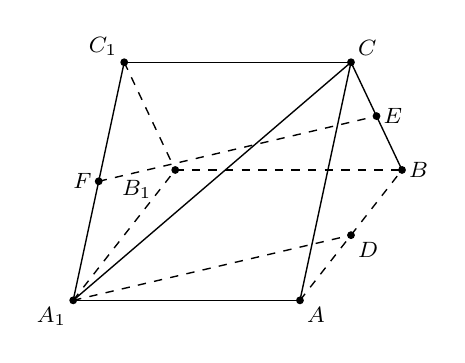
\begin{tikzpicture}[font=\footnotesize, line width=0.5pt, scale=0.72,
  dot/.style={circle, fill=black, inner sep=1.0pt}]
  \coordinate (A1) at (0,0);
  \coordinate (A)  at (4,0);
  \coordinate (C1) at (0.9,4.2);
  \coordinate (C)  at (4.9,4.2);
  \coordinate (B)  at (5.8,2.3);
  \coordinate (B1) at (1.8,2.3);
  \coordinate (D)  at (4.9,1.15);
  \coordinate (E)  at (5.35,3.25);
  \coordinate (F)  at (0.45,2.1);
  % 可见棱与可见面上的辅助线
  \draw (A1) -- (A);
  \draw (A) -- (C);
  \draw (C) -- (C1);
  \draw (C1) -- (A1);
  \draw (C) -- (B);
  \draw (A1) -- (C);
  % 不可见棱与内部辅助线
  \draw[dashed] (A) -- (B);
  \draw[dashed] (B1) -- (B);
  \draw[dashed] (C1) -- (B1);
  \draw[dashed] (A1) -- (B1);
  \draw[dashed] (A1) -- (D);
  \draw[dashed] (F) -- (E);
  \foreach \p in {A,B,C,A1,B1,C1,D,E,F} \node[dot] at (\p) {};
  \node[above left=-1pt] at (C1) {$C_1$};
  \node[above right=-1pt] at (C) {$C$};
  \node[below left=-1pt] at (A1) {$A_1$};
  \node[below right=-1pt] at (A) {$A$};
  \node[right=-1pt] at (B) {$B$};
  \node[left=5pt, yshift=-7pt] at (B1) {$B_1$};
  \node[below right=-1pt] at (D) {$D$};
  \node[right=-1pt] at (E) {$E$};
  \node[left=-1pt] at (F) {$F$};
\end{tikzpicture}
\end{center}
\nopagebreak[4]
\Needspace{4\baselineskip}
\textbf{解析}
由 $A_1A\perp$ 底面 $ABC$ 知该棱柱为直棱柱；各棱长均相等，不妨设棱长为 $2$（长度整体缩放不影响所证关系与所成角）。

\Needspace{5\baselineskip}
以 $A$ 为原点，$AB$ 所在直线为 $x$ 轴，底面内过 $A$ 且垂直于 $AB$ 的直线为 $y$ 轴，$AA_1$ 为 $z$ 轴，建立空间直角坐标系。则
\nopagebreak[4]
\[A(0,0,0),\quad B(2,0,0),\quad C(1,\sqrt3,0),\quad A_1(0,0,2),\quad B_1(2,0,2),\quad C_1(1,\sqrt3,2).\]
\Needspace{5\baselineskip}
由中点坐标公式
\nopagebreak[4]
\[D(1,0,0),\qquad E\left(\frac32,\frac{\sqrt3}2,0\right),\qquad F\left(\frac12,\frac{\sqrt3}2,2\right).\]

\Needspace{5\baselineskip}
\textbf{（1）} 计算
\nopagebreak[4]
\[\overrightarrow{EF}=\left(-1,0,2\right).\]
\Needspace{5\baselineskip}
平面 $A_1CD$ 内两向量
\nopagebreak[4]
\[\overrightarrow{DC}=(0,\sqrt3,0),\qquad\overrightarrow{DA_1}=(-1,0,2),\]
\Needspace{5\baselineskip}
其法向量
\nopagebreak[4]
\[\mathbf n=\overrightarrow{DC}\times\overrightarrow{DA_1}=(2\sqrt3,\ 0,\ \sqrt3).\]
\Needspace{5\baselineskip}
于是 $\overrightarrow{EF}\cdot\mathbf n=-2\sqrt3+0+2\sqrt3=0$，即 $EF$ 平行于平面 $A_1CD$（或在其内）。又
\nopagebreak[4]
\[\overrightarrow{DE}\cdot\mathbf n=2\left(\frac32-1\right)+0=\sqrt3\neq0,\]
故 $E\notin$ 平面 $A_1CD$，从而 $EF\parallel$ 平面 $A_1CD$。

\Needspace{5\baselineskip}
\textbf{（2）} 平面 $A_1ABB_1$ 即 $y=0$ 平面，其法向量可取 $\mathbf m=(0,1,0)$。由（1）知平面 $A_1CD$ 的法向量 $\mathbf n=(2\sqrt3,0,\sqrt3)$，而
\nopagebreak[4]
\[\mathbf n\cdot\mathbf m=0,\]
故两平面的法向量互相垂直，即平面 $A_1CD\perp$ 平面 $A_1ABB_1$。

\Needspace{5\baselineskip}
\textbf{（3）} $\overrightarrow{BC}=(-1,\sqrt3,0)$，$|\overrightarrow{BC}|=2$，$|\mathbf n|=\sqrt{12+3}=\sqrt{15}$。设直线 $BC$ 与平面 $A_1CD$ 所成的角为 $\theta$，则
\nopagebreak[4]
\[\sin\theta=\frac{|\overrightarrow{BC}\cdot\mathbf n|}{|\overrightarrow{BC}|\cdot|\mathbf n|}
=\frac{|{-2\sqrt3}|}{2\sqrt{15}}=\frac{\sqrt3}{\sqrt{15}}=\frac1{\sqrt5}=\frac{\sqrt5}5.\]
故所求正弦值为 $\dfrac{\sqrt5}5$。

\gkanswer{答案（1）：证明见解析。}

\gkanswer{答案（2）：证明见解析。}

\gkanswer{答案（3）：$\dfrac{\sqrt5}5$。}

\end{answer}
\begin{answer}
\gksolhead{18}{}

\textbf{题目}：

设椭圆 $\dfrac{x^2}{a^2}+\dfrac{y^2}{b^2}=1$（$a>b>0$）的左焦点为 $F$，离心率为 $\dfrac{\sqrt3}3$，过点 $F$ 且与 $x$ 轴垂直的直线被椭圆截得的线段长为 $\dfrac{4\sqrt3}3$。

（1） 求椭圆的方程；

（2） 设 $A$，$B$ 分别为椭圆的左、右顶点，过点 $F$ 且斜率为 $k$ 的直线与椭圆交于 $C$，$D$ 两点。若 $\overrightarrow{AC}\cdot\overrightarrow{DB}+\overrightarrow{AD}\cdot\overrightarrow{CB}=8$，求 $k$ 的值。

\Needspace{4\baselineskip}
\textbf{解析}
\Needspace{5\baselineskip}
\textbf{（1）} 设焦距参数 $c=\sqrt{a^2-b^2}$，则 $e=\dfrac ca=\dfrac{\sqrt3}3$，即 $c^2=\dfrac{a^2}3$，从而
\nopagebreak[4]
\[b^2=a^2-c^2=\frac{2a^2}3.\]
\Needspace{5\baselineskip}
过焦点 $F(-c,0)$ 且与 $x$ 轴垂直的直线为 $x=-c$，代入椭圆方程得
\nopagebreak[4]
\[\frac{c^2}{a^2}+\frac{y^2}{b^2}=1\Longrightarrow\frac{y^2}{b^2}=1-\frac13=\frac23\Longrightarrow y=\pm\frac{\sqrt6}3b,\]
\Needspace{5\baselineskip}
故截得线段长为 $\dfrac{2\sqrt6}3b$。由题设
\nopagebreak[4]
\[\frac{2\sqrt6}3b=\frac{4\sqrt3}3\Longrightarrow b=\frac{4\sqrt3}{3}\cdot\frac3{2\sqrt6}=\frac{2\sqrt3}{\sqrt6}=\sqrt2.\]
\Needspace{5\baselineskip}
于是 $b^2=2$，$a^2=\dfrac32b^2=3$，$c=1$。椭圆方程为
\nopagebreak[4]
\[\frac{x^2}3+\frac{y^2}2=1.\]

\Needspace{5\baselineskip}
\textbf{（2）} 由（1）$F(-1,0)$，$A(-\sqrt3,0)$，$B(\sqrt3,0)$。过 $F$ 且斜率为 $k$ 的直线为
\nopagebreak[4]
\[y=k(x+1).\]
\Needspace{5\baselineskip}
代入椭圆方程 $2x^2+3y^2=6$：
\nopagebreak[4]
\[2x^2+3k^2(x+1)^2=6\Longrightarrow(2+3k^2)x^2+6k^2x+3k^2-6=0.\]
\Needspace{5\baselineskip}
设 $C(x_1,y_1)$，$D(x_2,y_2)$，由韦达定理
\nopagebreak[4]
\[x_1+x_2=-\frac{6k^2}{2+3k^2},\qquad x_1x_2=\frac{3k^2-6}{2+3k^2}.\]
\Needspace{5\baselineskip}
又 $y_i=k(x_i+1)$，故
\nopagebreak[4]
\[\begin{aligned}
y_1y_2&=k^2(x_1+1)(x_2+1)=k^2\left(x_1x_2+x_1+x_2+1\right)\\
&=k^2\cdot\frac{(3k^2-6)+(-6k^2)+(2+3k^2)}{2+3k^2}=-\frac{4k^2}{2+3k^2}.
\end{aligned}\]
\Needspace{5\baselineskip}
由 $A(-\sqrt3,0)$，$B(\sqrt3,0)$ 得
\nopagebreak[4]
\[\overrightarrow{AC}=(x_1+\sqrt3,\ y_1),\quad\overrightarrow{DB}=(\sqrt3-x_2,\ -y_2),\]
\nopagebreak[4]
\[\overrightarrow{AD}=(x_2+\sqrt3,\ y_2),\quad\overrightarrow{CB}=(\sqrt3-x_1,\ -y_1).\]
\Needspace{5\baselineskip}
于是
\nopagebreak[4]
\[\overrightarrow{AC}\cdot\overrightarrow{DB}=(x_1+\sqrt3)(\sqrt3-x_2)-y_1y_2,\qquad
\overrightarrow{AD}\cdot\overrightarrow{CB}=(x_2+\sqrt3)(\sqrt3-x_1)-y_1y_2.\]
\Needspace{5\baselineskip}
两式相加，一次项相消：
\nopagebreak[4]
\[\overrightarrow{AC}\cdot\overrightarrow{DB}+\overrightarrow{AD}\cdot\overrightarrow{CB}=6-2x_1x_2-2y_1y_2=6-2(x_1x_2+y_1y_2).\]
\Needspace{5\baselineskip}
而
\nopagebreak[4]
\[x_1x_2+y_1y_2=\frac{3k^2-6-4k^2}{2+3k^2}=-\frac{k^2+6}{2+3k^2},\]
\Needspace{5\baselineskip}
故原式 $=6+\dfrac{2(k^2+6)}{2+3k^2}$。令其等于 $8$：
\nopagebreak[4]
\[\frac{2(k^2+6)}{2+3k^2}=2\Longrightarrow k^2+6=2+3k^2\Longrightarrow k^2=2\Longrightarrow k=\pm\sqrt2.\]
当 $k^2=2$ 时方程 $(2+3k^2)x^2+6k^2x+3k^2-6=0$ 即 $8x^2+12x=0$，有两不等实根，符合题意。故 $k=\pm\sqrt2$。

\gkanswer{答案（1）：$\dfrac{x^2}3+\dfrac{y^2}2=1$。}

\gkanswer{答案（2）：$k=\pm\sqrt2$。}

\end{answer}
\begin{answer}
\gksolhead{19}{}

\textbf{题目}：

已知首项为 $\dfrac32$ 的等比数列 $\{a_n\}$ 的前 $n$ 项和为 $S_n$（$n\in\mathbf N^*$），且 $-2S_2$，$S_3$，$4S_4$ 成等差数列。

（1） 求数列 $\{a_n\}$ 的通项公式；

（2） 证明 $S_n+\dfrac1{S_n}\leqslant\dfrac{13}6$（$n\in\mathbf N^*$）。

\Needspace{4\baselineskip}
\textbf{解析}
\Needspace{5\baselineskip}
\textbf{（1）} 设公比为 $q$。等比数列要求 $q\neq0$，且
\nopagebreak[4]
\[S_2=a_1(1+q),\quad S_3=a_1(1+q+q^2),\quad S_4=a_1(1+q+q^2+q^3).\]
\Needspace{5\baselineskip}
由 $-2S_2$，$S_3$，$4S_4$ 成等差数列得 $2S_3=-2S_2+4S_4$，即
\nopagebreak[4]
\[2a_1(1+q+q^2)=-2a_1(1+q)+4a_1(1+q+q^2+q^3).\]
\Needspace{5\baselineskip}
由 $a_1=\dfrac32\neq0$，两边约去 $2a_1$：
\nopagebreak[4]
\[1+q+q^2=-(1+q)+2(1+q+q^2+q^3)=1+q+2q^2+2q^3.\]
\Needspace{5\baselineskip}
移项得 $q^2+2q^3=0$，即 $q^2(1+2q)=0$。因 $q\neq0$，故 $q=-\dfrac12$。于是
\nopagebreak[4]
\[a_n=a_1q^{n-1}=\frac32\left(-\frac12\right)^{n-1}=\frac{3(-1)^{n-1}}{2^n}\quad(n\in\mathbf N^*).\]

\Needspace{5\baselineskip}
\textbf{（2）} 由（1）及等比数列求和公式（$q=-\dfrac12\neq1$）：
\nopagebreak[4]
\[S_n=\frac{a_1(1-q^n)}{1-q}=\frac{\frac32\left[1-\left(-\frac12\right)^n\right]}{1+\frac12}=1-\left(-\frac12\right)^n.\]
\Needspace{5\baselineskip}
因 $\left|\left(-\frac12\right)^n\right|\leqslant\dfrac12<1$，故 $S_n>0$，且
\nopagebreak[4]
\[S_n=\begin{cases}1+2^{-n}, & n\ \text{\text{为奇数}},\\[2pt] 1-2^{-n}, & n\ \text{\text{为偶数}}.\end{cases}\]

\Needspace{5\baselineskip}
当 $n$ 为奇数时，$S_n\in\left(1,\dfrac32\right]$。函数 $u+\dfrac1u$ 在 $[1,+\infty)$ 上单调递增，故
\nopagebreak[4]
\[S_n+\frac1{S_n}\leqslant\frac32+\frac23=\frac{13}6,\]
等号在 $n=1$ 时成立。

\Needspace{5\baselineskip}
当 $n$ 为偶数时，$S_n\in\left[\dfrac34,1\right)$。函数 $u+\dfrac1u$ 在 $(0,1]$ 上单调递减，故
\nopagebreak[4]
\[S_n+\frac1{S_n}\leqslant\frac34+\frac43=\frac{25}{12}<\frac{13}6.\]

综上，对一切 $n\in\mathbf N^*$ 都有 $S_n+\dfrac1{S_n}\leqslant\dfrac{13}6$。

\gkanswer{答案（1）：$a_n=\dfrac32\left(-\dfrac12\right)^{n-1}$（$n\in\mathbf N^*$）。}

\gkanswer{答案（2）：证明见解析。}

\end{answer}
\begin{answer}
\gksolhead{20}{}

\textbf{题目}：

设 $a\in[-2,0]$，已知函数 $f(x)=\begin{cases}x^3-(a+5)x, & x\leqslant0,\\ x^3-\dfrac{a+3}2x^2+ax, & x>0.\end{cases}$

（1） 证明：$f(x)$ 在区间 $(-1,1)$ 内单调递减，在区间 $(1,+\infty)$ 内单调递增；

（2） 设曲线 $y=f(x)$ 在点 $P_i(x_i,f(x_i))$（$i=1$，$2$，$3$）处的切线相互平行，且 $x_1x_2x_3\neq0$，证明：$x_1+x_2+x_3>-\dfrac13$。

\Needspace{4\baselineskip}
\textbf{解析}
\Needspace{5\baselineskip}
\textbf{（1）} 当 $x<0$ 时，
\nopagebreak[4]
\[f'(x)=3x^2-(a+5).\]
由 $a\in[-2,0]$ 得 $a+5\in[3,5]$。当 $|x|<1$ 时 $3x^2<3\leqslant a+5$，故 $f'(x)<0$，即 $f$ 在 $(-1,0]$ 上单调递减。

\Needspace{5\baselineskip}
当 $x>0$ 时，
\nopagebreak[4]
\[f'(x)=3x^2-(a+3)x+a=(3x-a)(x-1).\]
\Needspace{5\baselineskip}
因 $a\leqslant0$ 且 $x>0$，有 $3x-a>0$，故 $f'(x)$ 的符号由 $x-1$ 决定：
\nopagebreak[4]
\[0<x<1\ \text{\text{时}}\ f'(x)<0;\qquad x>1\ \text{\text{时}}\ f'(x)>0.\]
即 $f$ 在 $(0,1)$ 上单调递减，在 $(1,+\infty)$ 上单调递增。

又 $f$ 在 $x=0$ 处连续（两段在 $0$ 处的值均为 $0$），故 $f$ 在 $(-1,1)$ 内单调递减，在 $(1,+\infty)$ 内单调递增。

\textbf{（2）} 设三处切线的公共斜率为 $m$。

\Needspace{5\baselineskip}
先说明三个点中恰有一个横坐标为负。对 $x<0$，$f'(x)=3x^2-(a+5)$ 是偶函数且在 $(-\infty,0)$ 上单调递减，故方程 $f'(x)=m$ 即 $3x^2=m+a+5$ 在 $x<0$ 时至多有一个解；由 $x_1x_2x_3\neq0$ 及三切线平行知三点互异，故其中至少一个在 $x<0$ 上，从而恰有一个在 $x<0$ 上。不妨设
\nopagebreak[4]
\[x_3<0,\qquad x_1>0,\quad x_2>0.\]

\Needspace{5\baselineskip}
$x_1$，$x_2$ 是方程 $3x^2-(a+3)x+(a-m)=0$ 的两个正根，由韦达定理
\nopagebreak[4]
\[x_1+x_2=\frac{a+3}3,\qquad x_1x_2=\frac{a-m}3>0,\]
故 $m<a$。

\Needspace{5\baselineskip}
另一方面，由 $x_3<0$ 满足 $3x_3^2-(a+5)=m$ 得
\nopagebreak[4]
\[m+a+5=3x_3^2>0,\qquad |x_3|=\sqrt{\frac{m+a+5}3}.\]
\Needspace{5\baselineskip}
由 $m<a$ 得
\nopagebreak[4]
\[3(m+a+5)<3(2a+5)=6a+15=(a+4)^2-(a+1)^2\leqslant(a+4)^2,\]
\Needspace{5\baselineskip}
即
\nopagebreak[4]
\[\frac{m+a+5}3<\frac{(a+4)^2}9\Longrightarrow|x_3|<\frac{a+4}3\Longrightarrow x_3>-\frac{a+4}3,\]
\Needspace{5\baselineskip}
其中用到 $a+4>0$ 与 $m+a+5>0$，两边开方不等号方向不变。于是
\nopagebreak[4]
\[x_1+x_2+x_3>\frac{a+3}3-\frac{a+4}3=-\frac13,\]
即 $x_1+x_2+x_3>-\dfrac13$。

\gkanswer{答案（1）：证明见解析。}

\gkanswer{答案（2）：证明见解析。}

\end{answer}